\chapter{Results}

\section{Performance of GPU tridiagonal solver}

In this section we present a performance overview
of our NEATO solver
against a multi-threaded Intel MKL solver and
the CUSPARSE GPU solver
(\texttt{dgtsv} and \texttt{dgtsvStridedBatch} respectively).
The MKL solver uses Gaussian elimination with partial pivoting,
and the CUSPARSE solver uses a combination of
Cyclic Reduction and Parallel Cyclic Reduction
as described by Zhang et al. \cite{Zhang2010FTS}.
These solvers represent the most straightforward way
to compute solutions for tridiagonal systems
and are highly optimized for performance on
underlying architectures.
Boundary conditions may prevent
the matrix from being symmetric and/or diagonally dominant,
precluding the use of more specialized tridiagonal solvers.

The CPU code is compiled with the Intel C compiler (version 15.0),
and run (with OpenMP support) on up to
16 independent cores of the the same shared-memory node
(one thread per core).
The CPU is an
Intel Xeon Processor E5-2670 v2 (2.50 GHz, 25 MB Smart Cache).
GPU code is compiled with the CUDA toolkit (version 6.5.14),
and run on the
NVIDIA Tesla K20 Accelerator.
When measuring GPU performance (both CUSPARSE and NEATO),
we do \emph{not} include the cost
of data transfer between the CPU and GPU.
This is because the tridiagonal solver is expected to be
part of a larger application.
This is in keeping with the timing strategies
in related literature.

The \texttt{-O2} level compiler optimizations are turned on for both
CPU and GPU code;
no further optimization options are enabled in either case.
Of course, we use double precision for all solvers.
The timings reported are
kernel \emph{execution} times, i.e.,
the time for all kernel(s) to execute completely
before returning the program control to the CPU.
All timings are averaged over 100 tridiagonal solves.

\subsection{NEATO: global memory v/s shared memory performance}

\begin{figure}[h]
\begin{center}
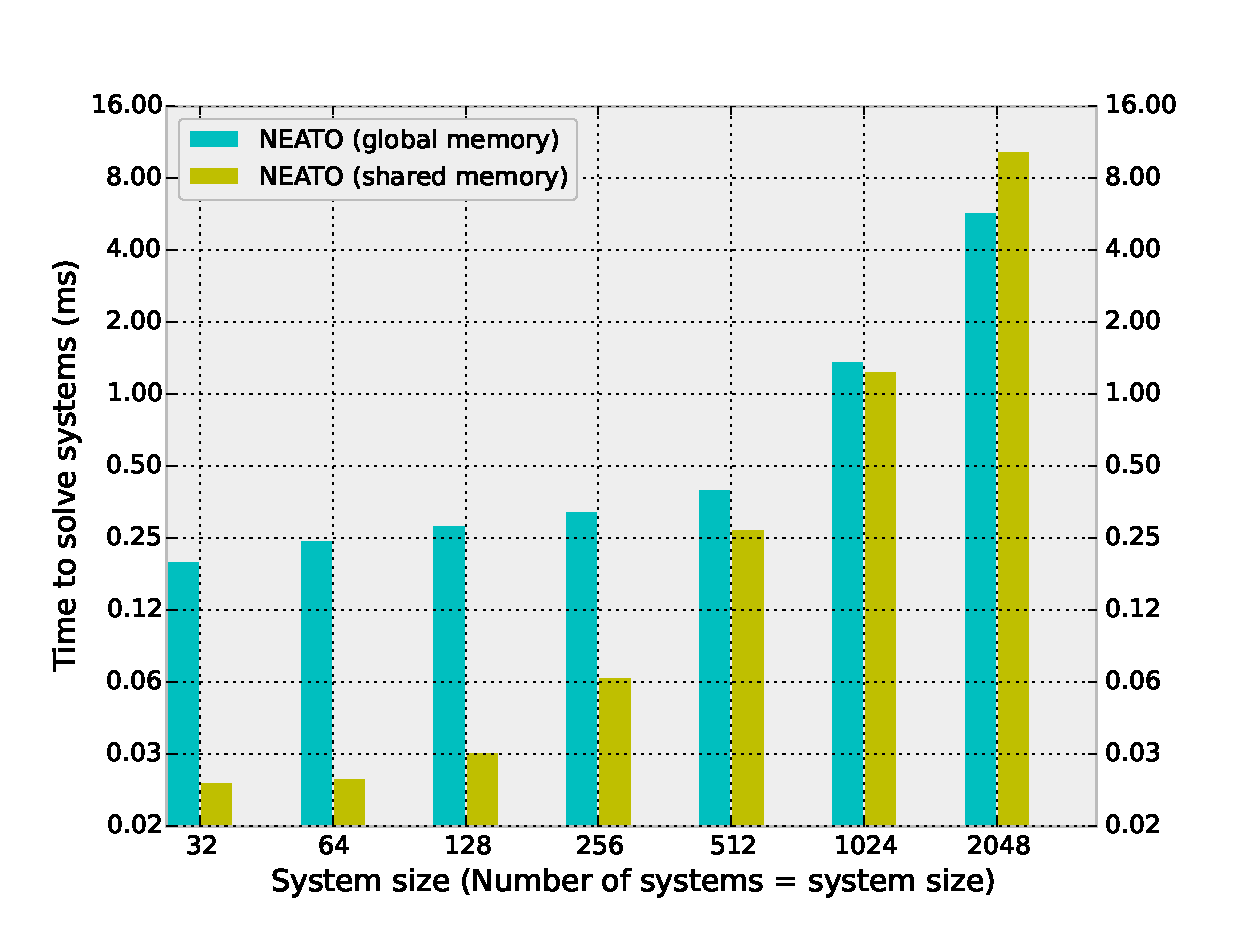
\includegraphics[width=300pt]{fig/global-vs-shared-2d.eps}
\caption{Comparison of global memory and shared
    memory implementations of NEATO (2D problems).}
\label{fig:global-vs-shared-2d}
\end{center}
\end{figure}

\begin{figure}[h]
\begin{center}
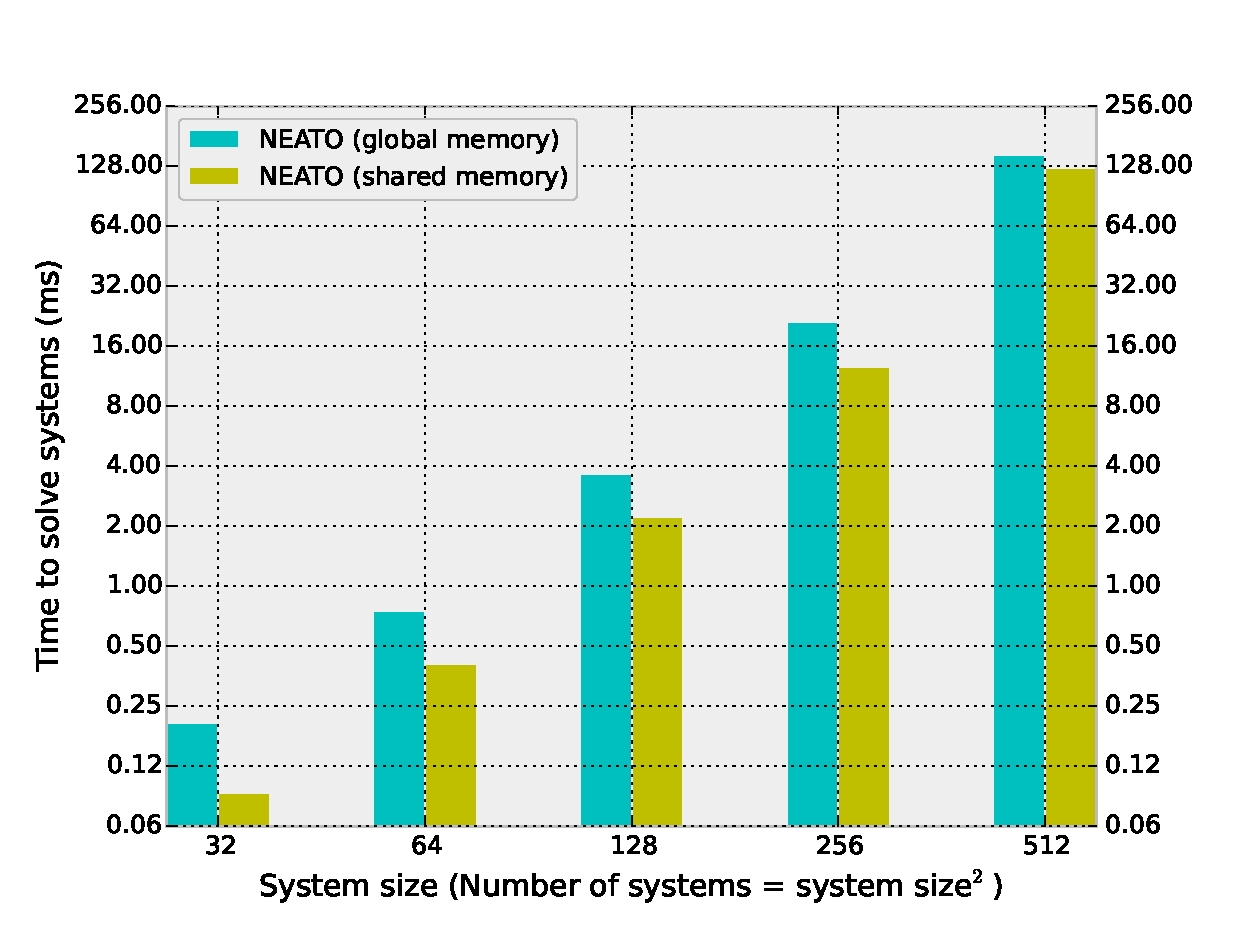
\includegraphics[width=300pt]{fig/global-vs-shared-3d.eps}
\caption{Comparison of global memory and shared memory
    implementations of NEATO (3D problems).}
\label{fig:global-vs-shared-3d}
\end{center}
\end{figure}

In Figs. \ref{fig:global-vs-shared-2d} and \ref{fig:global-vs-shared-3d},
we report the performance of the two solvers for the case
$N_{rhs} = n$ and $N_{rhs} = n^2$.
These cases correspond to tridiagonal systems
arising in 2-D and 3-D problems respectively.
We note that the shared memory implementation
offers better performance in nearly all cases.
However, the relative speedup from using
shared memory diminishes with increasing problem size.
For larger problem sizes,
the synchronization costs associated with inactive threads
leads to poor shared memory performance.

\subsection{Comparison of NEATO with Intel MKL and CUSPARSE solvers}

\begin{figure}
\begin{center}
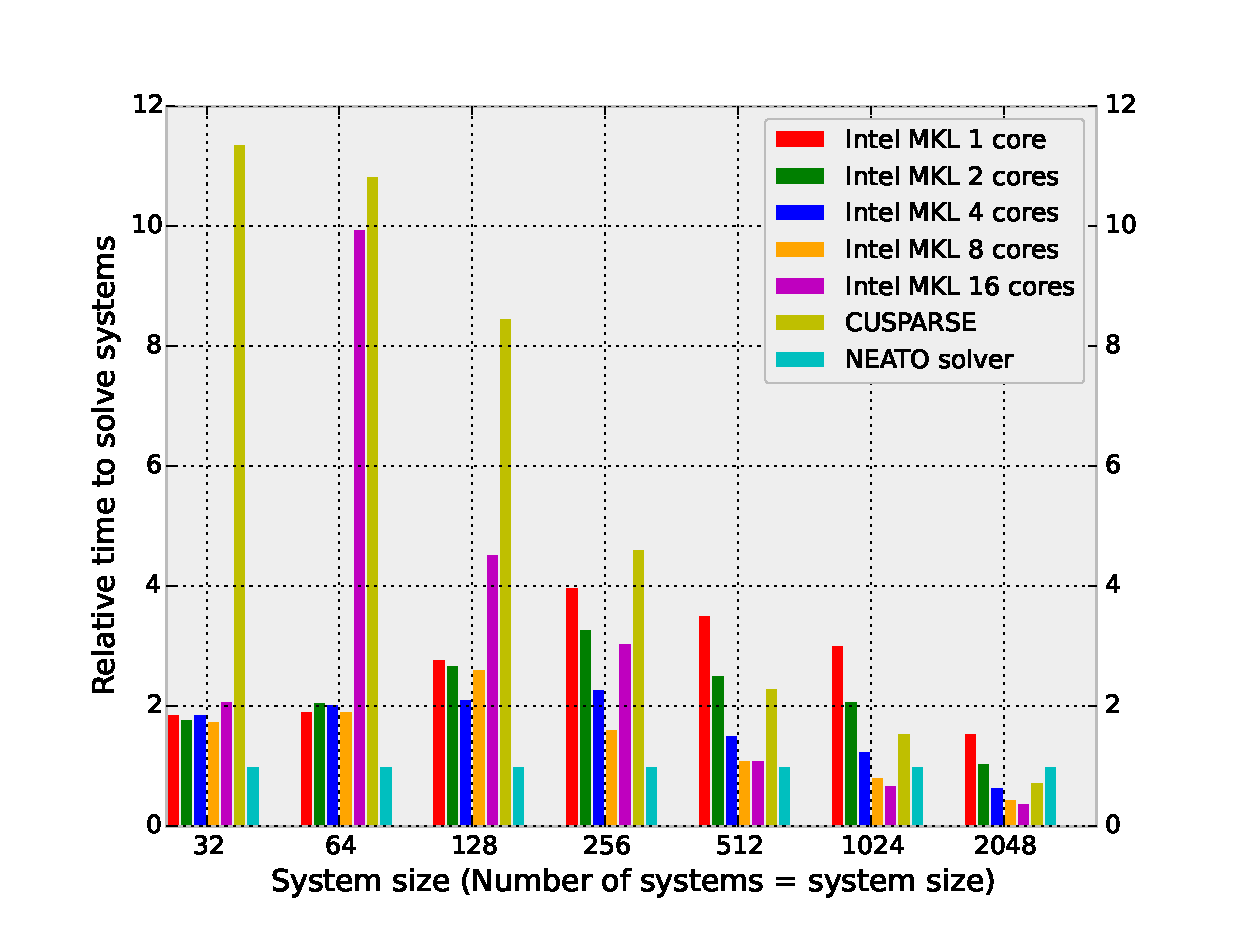
\includegraphics[width=300pt]{fig/bench-2d.eps}
\caption{Relative solver performance for 2-D problems. Relative time defined as:}
Time taken by solver/Time taken by NEATO solver
\label{fig:bench-2d}
\end{center}
\end{figure}

\begin{figure}
\begin{center}
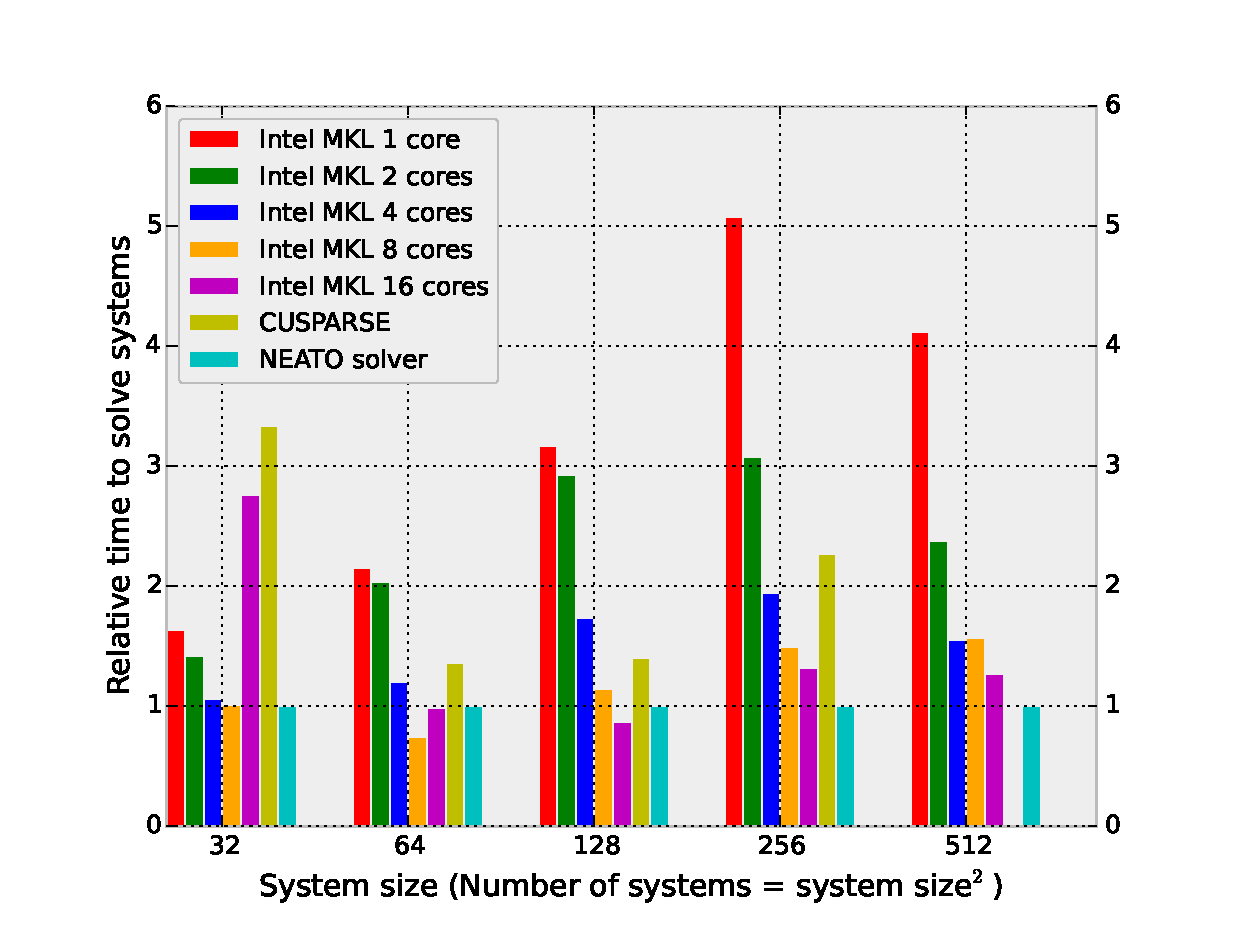
\includegraphics[width=300pt]{fig/bench-3d.eps}
\caption{Relative solver performance for 3-D problems. Relative time defined as:}
Time taken by solver/Time taken by NEATO solver
\label{fig:bench-3d}
\end{center}
\end{figure}

In Fig. \ref{fig:bench-2d} and \ref{fig:bench-3d},
we provide the relative performance of
Intel MKL and CUSPARSE solvers and compare against
the NEATO shared memory implementation.
The relative performance for
each problem size is obtained by
normalizing the solver timings
by the timing for the NEATO solver for that problem size.
Table \ref{table:bench} shows the timings of the various
solvers to solve different problem sizes.
Note that data is missing for the CUSPARSE solver
for the $512^3$ 3-D case,
as the GPU was unable to accomodate this problem size---this
is due to the large amount of scratch space required
by the CUSPARSE implementation.

\begin{sidewaystable}[]
\scriptsize
\centering
\caption{Performance of Intel MKL, CUSPARSE and NEATO solvers.}
\label{table:bench}
% Please add the following required packages to your document preamble:
% \usepackage{multirow}
\begin{tabular}{|l|l|l|l|l|l|l|}
\hline
\multirow{2}{*}              & \multirow{2}{*}{}        & \multicolumn{5}{c|}{Time to solve (ms)}                             \\ \cline{3-7}
\centering System size       & Number of systems        & MKL 1 core    & MKL 16 cores & CUSPARSE & NEATO (global) & NEATO (shared) \\ \hline
32                           & 32                       & 0.045         & 0.05         & 0.273    & 0.201          & 0.024          \\ \hline
64                           & 64                       & 0.048         & 0.249        & 0.271    & 0.247          & 0.025          \\ \hline
128                          & 128                      & 0.089         & 0.145        & 0.271    & 0.284          & 0.032          \\ \hline
256                          & 256                      & 0.263         & 0.202        & 0.305    & 0.326          & 0.066          \\ \hline
512                          & 512                      & 0.959         & 0.299        & 0.629    & 0.403          & 0.272          \\ \hline
1024                         & 1024                     & 3.775         & 0.864        & 1.939    & 1.375          & 1.252          \\ \hline
2048                         & 2048                     & 16.272        & 4.111        & 7.607    & 5.811          & 10.407         \\ \hline
32                           & 1024                     & 0.152         & 0.257        & 0.31     & 0.207          & 0.092          \\ \hline
64                           & 4096                     & 0.879         & 0.403        & 0.556    & 0.751          & 0.409          \\ \hline
128                          & 16384                    & 7.052         & 1.931        & 3.128    & 3.669          & 2.225          \\ \hline
256                          & 65536                    & 63.858        & 17.61        & 28.495   & 21.148         & 12.565         \\ \hline
512                          & 262144                   & 515.792       & 159.394      &          & 145.34         & 125.311        \\ \hline 
\end{tabular}

\end{sidewaystable}

\section{Performance of compact finite difference application}

The timings for the
compact finite difference application
were measured on the
Clemson University Palmetto Cluster,
using NVIDIA Tesla K20 and K40 GPUs.
The K40 GPUs were used for the largest problem sizes.
Each compute node on the cluster is equipped with up to 2 GPUs,
and nodes are connected by 56 Gbps Infiniband interconnect.
We use Open MPI 1.8.1 configured with OpenFabrics support.

The timings reported are \emph{wall clock} times
with global synchronization between processes performed 
before and after evaluation of the derivatives.
All timings are averaged over 100 evaluations of the function derivatives
in each coordinate direction.
We make it clear that our reported
problem sizes represent the \emph{actual size of problem data}.
Although it may be considered sufficient to
run tests on a single line of processes
for measuring the compact finite difference solver performance,
we set up and solve the problem for the entire computational domain.
In the context of a larger simulation,
global synchronization between the processes
is typically performed before and after the evaluation of derivatives,
and it is important to consider the related overhead.

\subsection{Performance profiling}

\begin{figure}[h!]
\begin{center}
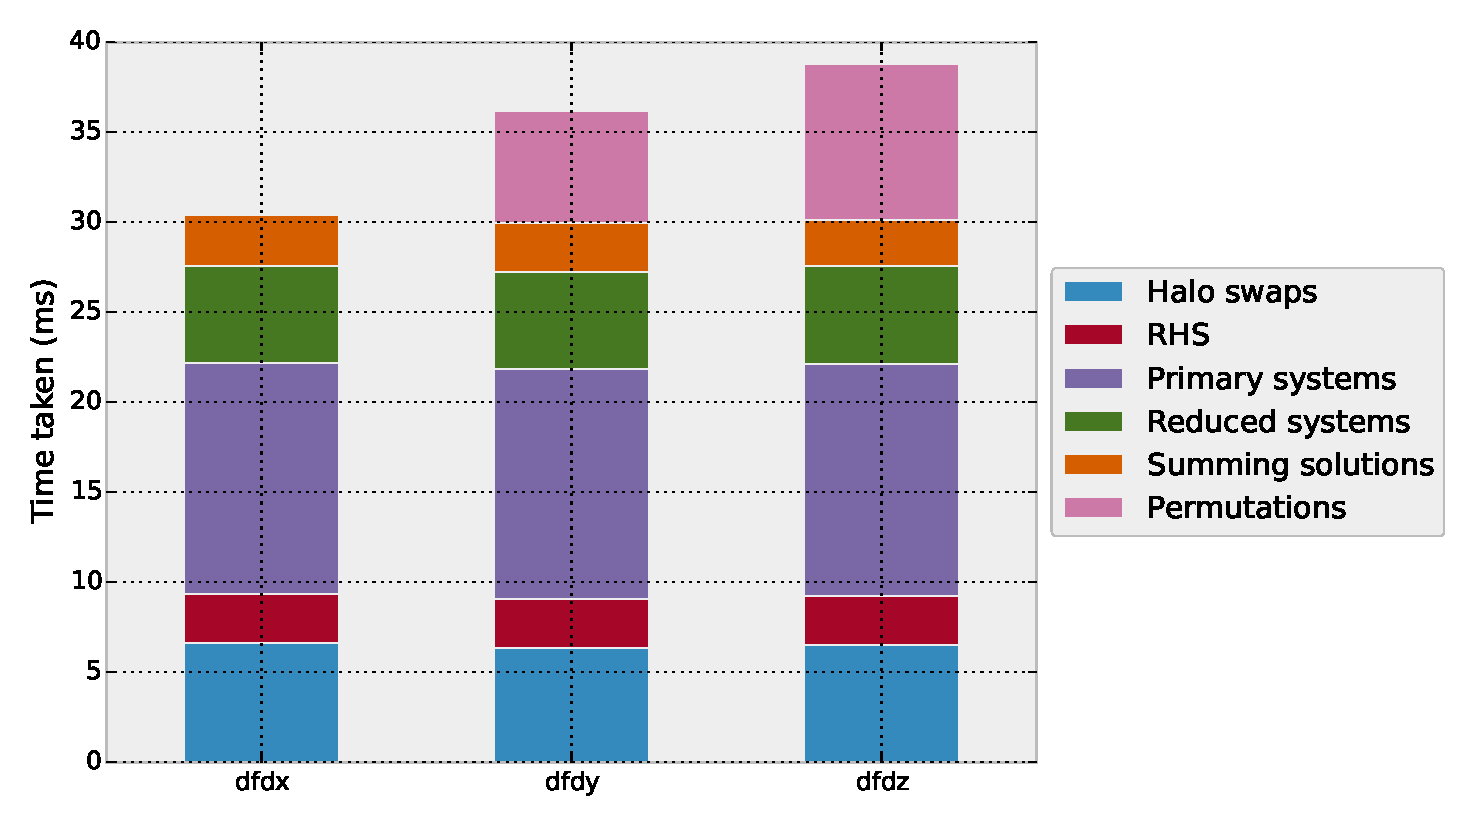
\includegraphics[width=300pt]{fig/profiling-1024-64.eps}
\caption{Solving problem sized $1024^3$ on 64 GPUs}
\label{fig:compact-profiling-1024-64}
\end{center}
\end{figure}
%
\begin{figure}[h!]
\begin{center}
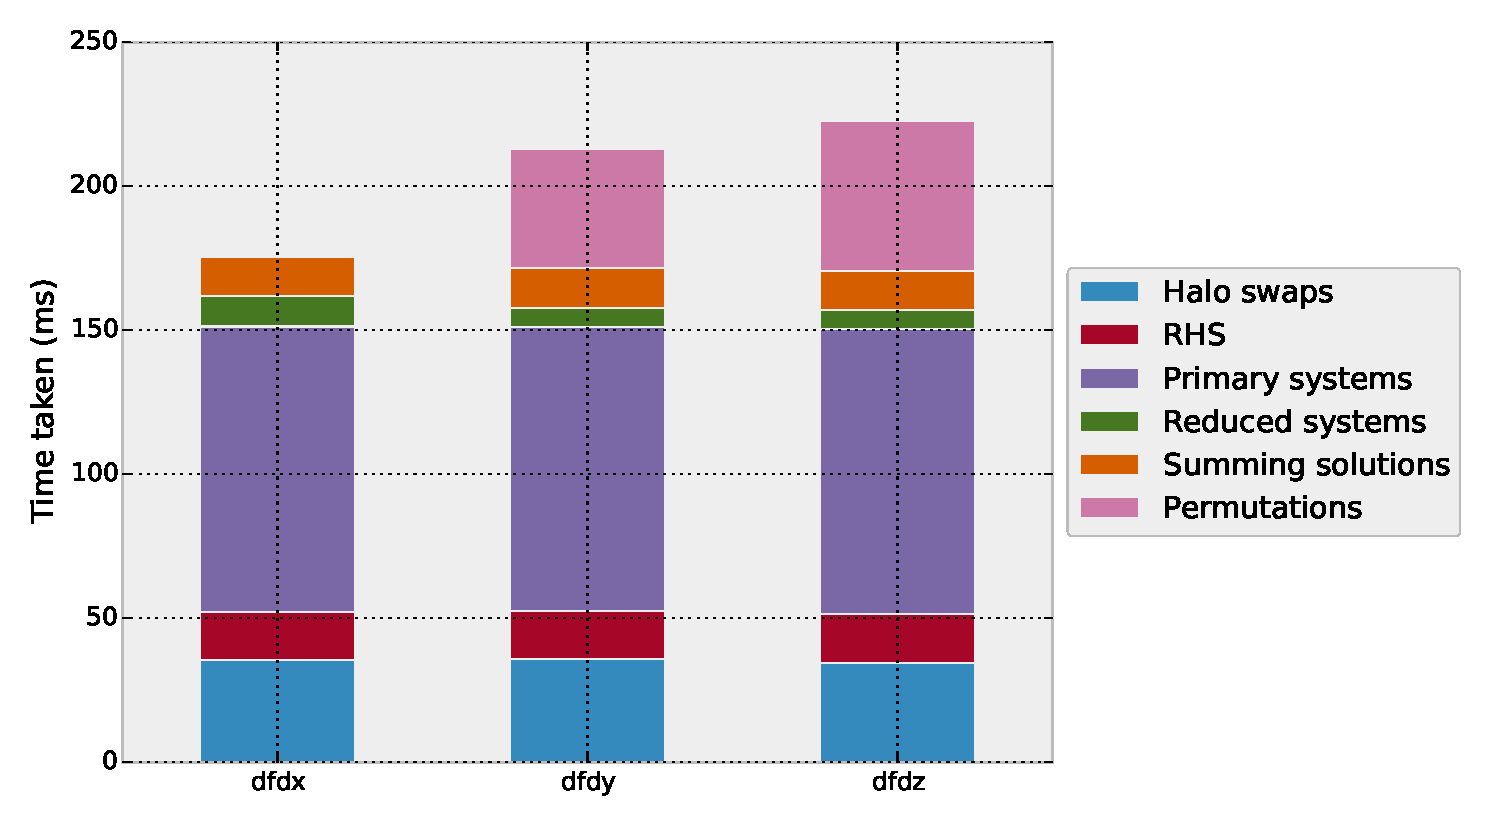
\includegraphics[width=300pt]{fig/profiling-2048-64.eps}
\caption{Solving problem sized $2048^3$ on 64 GPUs}
\label{fig:compact-profiling-2048-64}
\end{center}
\end{figure}
%
Figures \ref{fig:compact-profiling-1024-64} - \ref{fig:compact-profiling-2048-64}
show the time taken by the different steps of
the compact finite difference solver.
We note that for the larger problem size,
the evaluation of the primary systems (using the NEATO solver)
constitutes a larger majority of the total runtime,
which justifies our efforts in optimizing the tridiagonal solver.
For evaluation of the derivatives in the $y-$ and $z-$ directions,
we note that a significant portion of the runtime is dedicated
to performing permutations of the input and output data.
We attribute this to our na\"{\i}ve implementation of the
permutation kernels (no shared memory usage).

\subsection{Strong and weak scaling}
\begin{figure}
\begin{center}
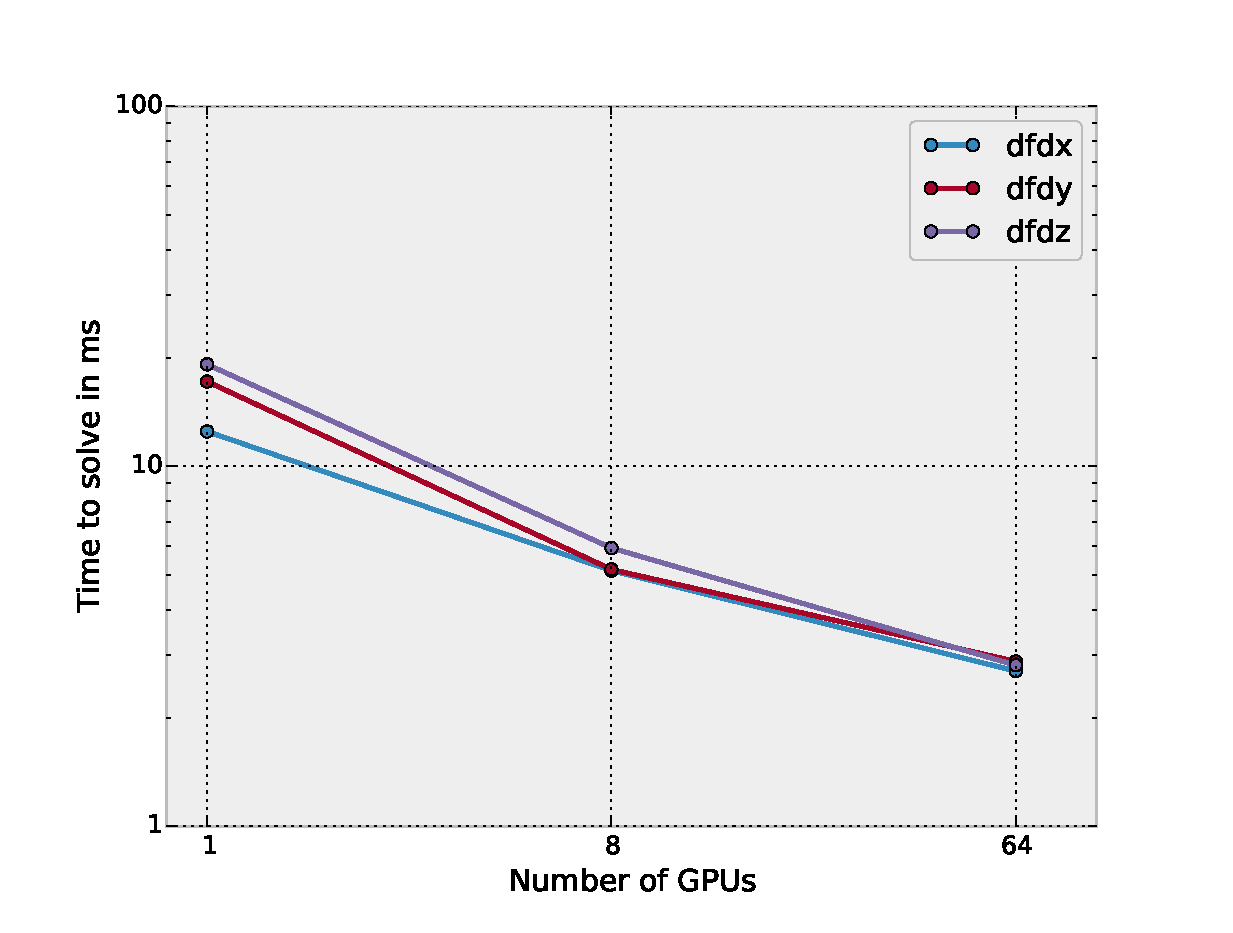
\includegraphics[width=300pt]{fig/strong-scaling-256.eps}
\caption{Strong scaling for multi-GPU compact finite difference, problem size: $256^3$.}
\label{fig:strong-scaling-256}
\end{center}
\end{figure}
%
\begin{figure}
\begin{center}
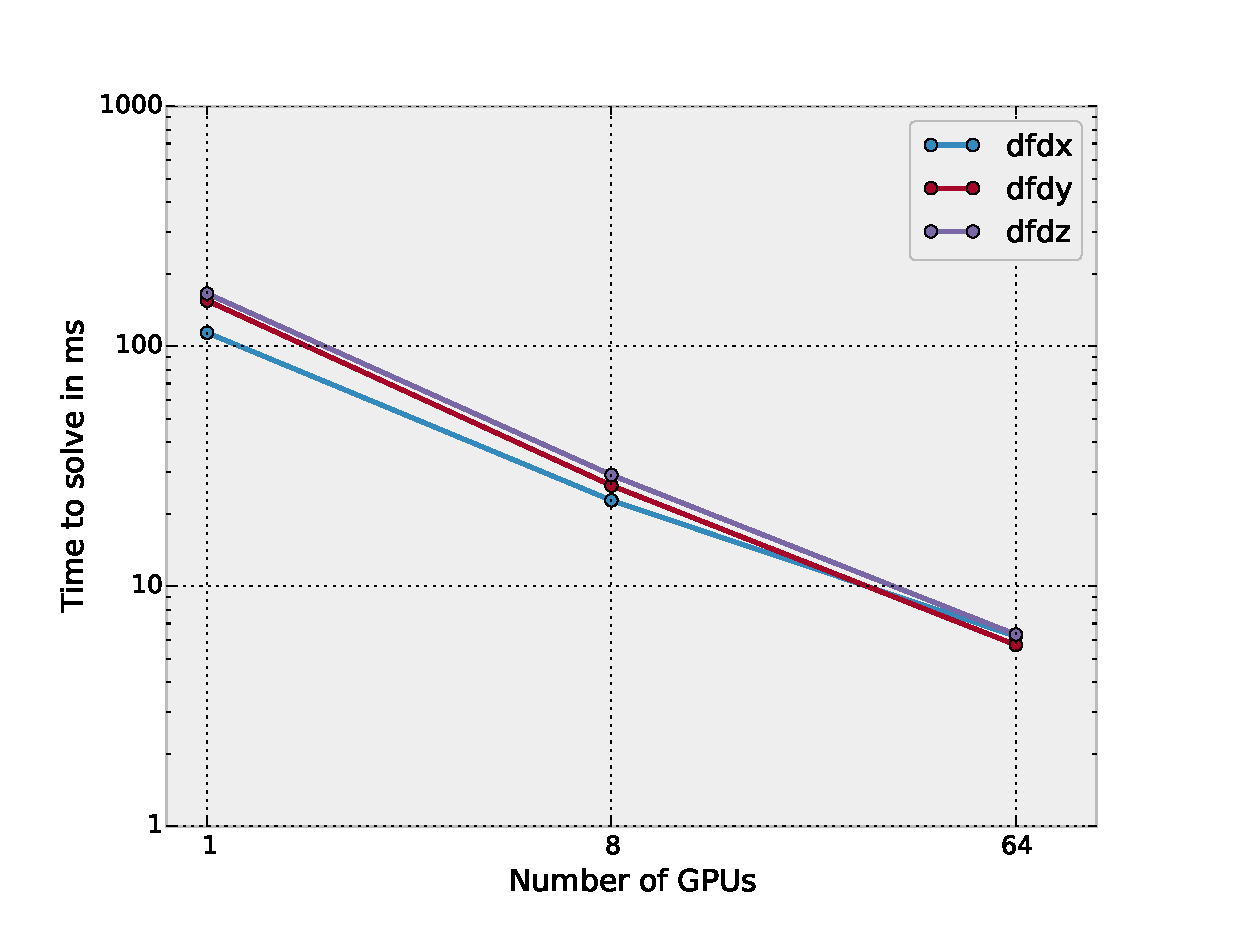
\includegraphics[width=300pt]{fig/strong-scaling-512.eps}
\caption{Strong scaling for multi-GPU compact finite difference, problem size: $512^3$.}
\label{fig:strong-scaling-512}
\end{center}
\end{figure}
%
\begin{figure}
\begin{center}
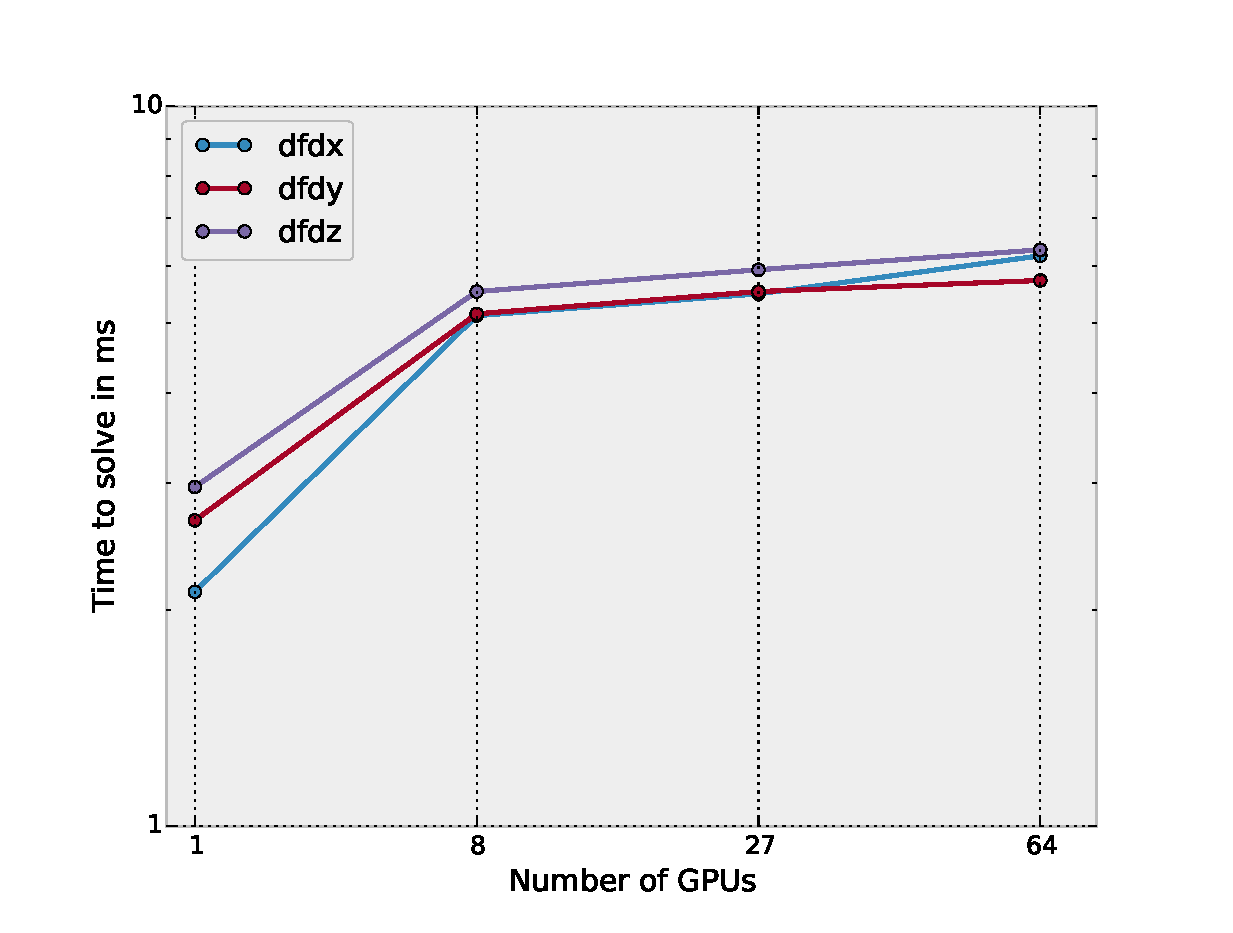
\includegraphics[width=300pt]{fig/weak-scaling-128.eps}
\caption{Weak scaling for multi-GPU compact finite difference, problem size: $128^3$ per process.}
\label{fig:weak-scaling-128}
\end{center}
\end{figure}
%
\begin{figure}
\begin{center}
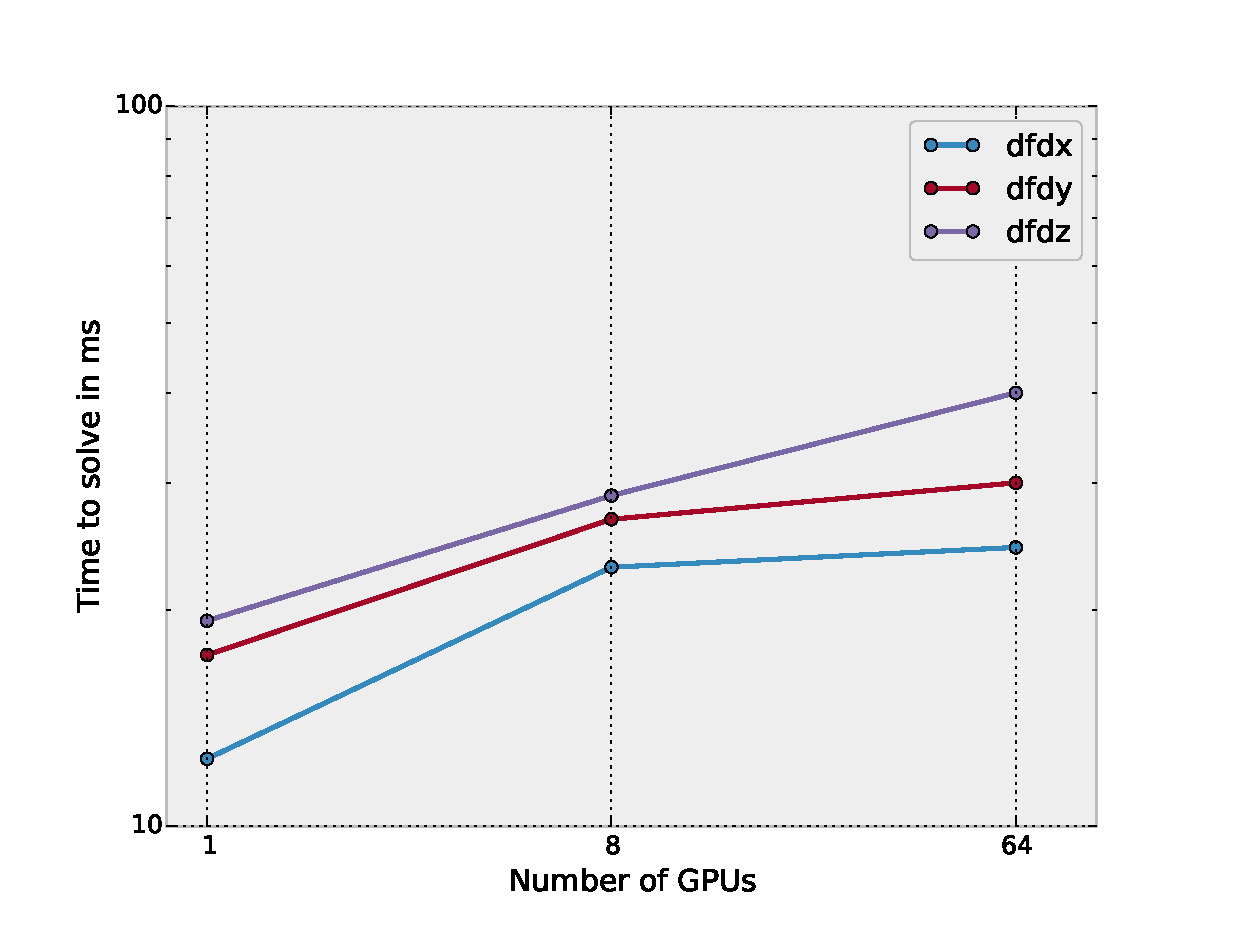
\includegraphics[width=300pt]{fig/weak-scaling-256.eps}
\caption{Weak scaling for multi-GPU compact finite difference, problem size: $256^3$ per process.}
\label{fig:weak-scaling-256}
\end{center}
\end{figure}
%
Figures \ref{fig:strong-scaling-256} - \ref{fig:weak-scaling-256}
show the strong and weak scaling of the compact finite difference solver
for evaluating derivatives in all three coordinate directions.
For the strong scaling measurement,
we keep the problem size fixed
and increase the number of GPUs used to solve the problem.
For the weak scaling measurement,
we keep the problem size \emph{per GPU}
fixed, and increase the number of GPUs used.
The strong scaling for larger problems is somewhat better
as the GPU is kept more busy.

\subsection{Comparison with a CPU-only approach}

\centering
\begin{tabular}{|l|l|l|l|l|l|l|}
\hline
\multirow{2}{*}{Size} & \multicolumn{3}{c|}{Ref. impl, \#CPU cores} & \multicolumn{3}{c|}{NEATO-based, \#GPUs} \\ \cline{2-7}
         & 8         & 64        & 512      & 1       & 8       & 64      \\ \hline
$256^3$  & 79.5      & 20.8      & 11.1     & 19.9    & 5.17    & 2.79    \\ \hline
$512^3$  & 556.8     & 146.5     & 29.2     & 164.5   & 23.24   & 5.62    \\ \hline
$1024^3$ & 5188      & 1092      & 223.7    & -       & 174.9   & 24.49   \\ \hline
$2048^3$ & -         & -         & 1741     & -       & -       & 297.07  \\ \hline
\end{tabular}

%
\begin{figure}
\begin{center}
\includegraphics[width=300pt]{fig/compact-refimpl-speedups.eps}
\caption{Speedups over reference implementation
    for computing derivative in the fastest coordinate direction}
\label{fig:compact-refimpl-speedups}
\end{center}
\end{figure}

We also compare the performance of our compact finite difference
solver with the approach described by
Mohd-Yusof et al.\ \cite{mohd2010adapting},
implemented for CPUs.
The approach uses a distributed tridiagonal solver based on
the LU decomposition specialized for tridiagonal systems.
The problem is divided among individual CPU cores,
communicating via MPI.
For comparing timings,
we use the number of CPU sockets as the basis.
Each CPU socket uses 8 CPU cores and 1 GPU.
Thus, we maintain a ratio of 1:8 between GPUs and CPU cores
in our comparison.
Table \ref{table:compact-refimpl-timings}
shows timings for computing derivatives
in the fastest coordinate direction
for problems sized up to $2048^3$,
and Fig. \ref{fig:compact-refimpl-speedups}
shows the respective speedup using our implementation.
